%%%%%%%%%%%%%%%%%%%%%%%%%%%%%%%%%%%%%%%%%
% Structured General Purpose Assignment
% LaTeX Template
%
% This template has been downloaded from:
% http://www.latextemplates.com
%
% Original author:
% Ted Pavlic (http://www.tedpavlic.com)
%
% Note:
% The \lipsum[#] commands throughout this template generate dummy text
% to fill the template out. These commands should all be removed when 
% writing assignment content.
%
%%%%%%%%%%%%%%%%%%%%%%%%%%%%%%%%%%%%%%%%%

%----------------------------------------------------------------------------------------
%   PACKAGES AND OTHER DOCUMENT CONFIGURATIONS
%----------------------------------------------------------------------------------------

\documentclass{article}

\usepackage{fancyhdr} % Required for custom headers
\usepackage{lastpage} % Required to determine the last page for the footer
\usepackage{extramarks} % Required for headers and footers
\usepackage{graphicx} % Required to insert images
\usepackage{lipsum} % Used for inserting dummy 'Lorem ipsum' text into the template

\usepackage[T1]{fontenc} % Codificación de las fuentes utilizadas
\usepackage[spanish]{babel} % Español como idioma principal del texto (permite hyphenation de palabras al final de una línea)
\selectlanguage{spanish}
\usepackage{hyperref}
\usepackage{listings}

\usepackage[T1]{fontenc} % Codificación de las fuentes utilizadas
\usepackage[spanish]{babel} % Español como idioma principal del texto (permite hyphenation de palabras al final de una línea)


\usepackage{graphicx}
\usepackage{url}

\graphicspath{{Figures/}{Diagrams}{Chapters/}}  % Location of the graphics files (set up for graphics to be in PDF format)

\selectlanguage{spanish}

\setcounter{tocdepth}{1}

% Include any extra LaTeX packages required
\usepackage[square, numbers, comma, sort&compress]{natbib}  % Use the "Natbib" style for the references in the Bibliography
\usepackage{verbatim}  % Needed for the "comment" environment to make LaTeX comments
\usepackage{vector}  % Allows "\bvec{}" and "\buvec{}" for "blackboard" style bold vectors in maths
\hypersetup{urlcolor=blue, colorlinks=true}  % Colours hyperlinks in blue, but this can be distracting if there are many links.
\usepackage{hyperref}
% \usepackage[pdfauthor={Diego Martín Arroyo},
%             pdftitle={Diseño e implementación de un sistema de computación distribuida con
% Raspberry Pi, y estudio comparativo del mismo frente a otras soluciones},
%             pdfsubject={Memora del Trabajo de Fin de Grado},
%             pdfproducer={XeLaTeX with hyperref},
%             pdfcreator={XeLaTeX},
%             pdfkeywords={Computación Paralela, Sistema Distribuido, Raspberry}
%             ]{hyperref}
%% ----------------------------------------------------------------

%% --------------------------------------------------------------------------------------------------------------------------------
%http://tex.stackexchange.com/a/85218/76599
\usepackage{fancyvrb}
\usepackage[dvipsnames]{xcolor}

% redefine \VerbatimInput
\RecustomVerbatimCommand{\VerbatimInput}{VerbatimInput}% Inclusión de archivos de texto plano
{fontsize=\footnotesize,
 %
 frame=lines,  % top and bottom rule only
 framesep=2em, % separation between frame and text
 rulecolor=\color{Gray},
 %
 label=\fbox{\color{Black}data.txt},
 labelposition=topline,
 %
 commandchars=\|\(\), % escape character and argument delimiters for
                      % commands within the verbatim
 commentchar=*        % comment character
}

\usepackage{listings} % Requerido para la inserción de código
%Listings command

\usepackage{float}
\newcommand*\lstinputpath[1]{\lstset{inputpath=#1}}
\lstinputpath{Code/}

\newcounter{undefinedreferences}
\setcounter{undefinedreferences}{0}

\newcommand{\citationneeded}[1][None]{\stepcounter{undefinedreferences}\textsuperscript{\color{blue} [Citation needed: #1]}}

\newcommand{\checkreferences}{
	\ifnum\value{undefinedreferences} > 0
	\begin{center}
		\immediate\write18{wget -O Figures/protester.png -nc http://imgs.xkcd.com/comics/wikipedian_protester.png}
		\includegraphics[width=\textwidth]{protester.png}\\
		There are \arabic{undefinedreferences} undefined references
	\end{center}
	\else
	No undefined references. Good!
	\fi
}


%https://github.com/pads-fhs/LaTeX-Template-Thesis/blob/master/lststyles.tex
\lstdefinelanguage{JavaScript}{
  keywords={typeof, new, true, false, catch,%
    function, return, null, catch, switch, var,%
    if, in, while, do, else, case, break},
  ndkeywords={class, export, boolean, throw, implements, import, this},
  sensitive=false,
  comment=[l]{//},
  morecomment=[s]{/*}{*/},
  morestring=[b]',
  morestring=[b]"
}
\newcommand{\lstsetjavascript}{
  \lstset{
		language=JavaScript,
		breaklines=true,
		commentstyle=\textit,
		basicstyle=\ttfamily,
		keywordstyle=\bfseries,
		stringstyle=\ttfamily,
		showstringspaces=false,
		frame=single,
		tabsize=2
  }
}

\lstdefinelanguage{log}{
  keywords={typeof, new, true, false, catch,%
    function, return, null, catch, switch, var,%
    if, in, while, do, else, case, break},
  ndkeywords={class, export, boolean, throw, implements, import, this},
  sensitive=false,
  comment=[l]{//},
  morecomment=[s]{/*}{*/},
  morestring=[b]',
  morestring=[b]"
}
\newcommand{\lstsetlog}{
  \lstset{
		language=log,
		breaklines=true,
		commentstyle=\textit,
		basicstyle=\ttfamily,
		keywordstyle=\bfseries,
		stringstyle=\ttfamily,
		showstringspaces=false,
		frame=single,
		tabsize=2
  }
}

\lstloadlanguages{Java,XML, JavaScript, log}

\newcommand{\javascriptcode}[4]{
	\lstinputlisting[caption=#2,label=#1, firstline=#3, lastline=#4]{#1.json}
}

\newcommand{\logcode}[4]{
	\lstinputlisting[caption=#2,label=#1, firstline=#3, lastline=#4]{#1.log}
}

\usepackage[bottom]{footmisc} %The footnotes go at the bottom of t\usepackage{dtklogos}he page, instead next to the last line.
%Ajustes para Java
% \lstset{
% 	language=java,
%  	frame=single, % Un marco simple alrededor del código
%     basicstyle=\small\ttfamily, % Utilizar fuente true type pequeña
%     keywordstyle=[1]\color{Blue}\bf, % Funciones en negrita y azul
%     keywordstyle=[2]\color{Purple}, % Argumentos en morado
%     keywordstyle=[3]\color{Blue}\underbar, % Funciones personalizadas subrayadas en azul
%     identifierstyle=, % Nada especial acerca de identificadores
%     commentstyle=\usefont{T1}{pcr}{m}{sl}\color{Green}\small, % Los comentarios se renderizan en fuente pequeña verde
%     stringstyle=\color{Purple}, % Cadenas en morado
%     showstringspaces=false, % No se muestran los espacios entre cadenas
%     tabsize=5, % 5 espacios por tabulado
%     %
%     % Put standard Perl functions not included in the default language here
%     %morekeywords={rand},
%     %
%     % Put Perl function parameters here
%     %morekeywords=[2]{on, off, interp},
%     %
%     % Put user defined functions here
%     %morekeywords=[3]{test},\usepackage{dtklogos}
%    	%
%     morecomment=[l][\color{Blue}]{...}, % Line continuation (...) like blue comment
%     numbers=left, % Número de línea a la izquierda
%     firstnumber=1, % Número de línea comienza en 1
%     numberstyle=\tiny\color{Blue}, % Los números de línea son azules y pequeños
%     stepnumber=5, % Los números de línea van de 5 en 5
%     breaklines=true % Salto de línea si el texto no entra. See http://stackoverflow.com/a/1875803
% }

%\usepackage{xltxtra} % XeLaTeX logo. Yep, just that
%http://tex.stackexchange.com/a/73179/76599
\usepackage{metalogo}
\usepackage{dtklogos} %BibTeX logo
\usepackage{float}
\usepackage{pdflscape}
%----------------------------------------------------------------------------------------
%   NAME AND CLASS SECTION
%----------------------------------------------------------------------------------------

\newcommand{\hmwkTitle}{Estructura física} % Assignment title
\newcommand{\hmwkDueDate}{Lunes,\ 6\ de\ julio\ de\ 2015} % Due date
\newcommand{\hmwkAuthorName}{Diego Martín Arroyo} % Your name

\graphicspath{{Figures/}}
%----------------------------------------------------------------------------------------
%   TITLE PAGE
%----------------------------------------------------------------------------------------

\title{\hmwkTitle}
\author{\textbf{\hmwkAuthorName}}
\date{\hmwkDueDate}

%----------------------------------------------------------------------------------------
\begin{document}

\maketitle
\begin{abstract}
Marcologger es una herramienta que permite observar la salida de un programa distribuido desde una única interfaz, integrándose además en rsyslog, utilizando Snorky para la gestión de los WebSockets.
\end{abstract}

%----------------------------------------------------------------------------------------
%   TABLE OF CONTENTS
%----------------------------------------------------------------------------------------

\setcounter{tocdepth}{1}

\tableofcontents
\newpage

\section{Introducción}

En el presente anexo se detallan todos los aspectos de relevancia de la estructura física final, sirviendo como referencia para conocer todo el proceso de desarrollo llevado a cabo y la replicación del producto final.

\section{Estructura}

\subsection{Soporte}

El soporte de todos los componentes está formado por una serie de placas de metacrilato que actuan a modo de baldas, sosteniendo los nodos. Estas placas se unen unas a otras mediante una serie de barras de latón.

Las placas de metacrilato han sido cortadas a mano a partir de una pieza y los tubos han sido fabricados cortando una barra del metal.

También se utiliza latón para el soporte de los nodos en cada una de las baldas, con pequeñas ``patas'' que sostienen en el aire cada una de las Rasbperries aprovechando los diferentes agujeros de los que disponen para este tipo de propósitos.

%TODO: foto

\subsubsection{Planos}

\subsection{Red}

Toda la red de datos está soportada por dos \textit{switches} TP-Link 10/100 que se sitúan en la parte inferior de la estructura. Los nodos se conectan a este componente a través de cables Ethernet UTP cortados y crimpados a medida manualmente.

\subsection{Alimentación eléctrica}

Uno de los aspectos más ingeniosos de la estructura es la gestión de la red eléctrica. La alimentación del sistema se centraliza en una fuente que provee de tensión continua a 5 V con una intensidad máxima de 20 amperios. La fuente se sitúa anexa a estantería principal y de ella parten diferentes cables de alimentación a cada uno de los componentes de la estructura, y a la conexión de corriente alterna que la alimenta, a través de un enchufe convencional.

Es resaltable el hecho de que todos los componentes de la estructura están conectados a esta fuente eléctrica. Se han modificado unos cables USB a micro-USB, pelando las cabezas micro-USB y soldando a estas dos cables de corriente que se dirigen a las tomas positiva y negativa de la fuente. La conexión con el \textit{switch} se realiza adquiriendo conectores de corriente continua (los utilizados por defecto por el equipo) y realizando el mismo proceso que para las cabezas USB.

%FOTO cables

Además de los mecanismos de protección con los que cuenta la fuente se incluye un fusible protector de 2 amperios por cada cable positivo.

\section{LED}

Los diferentes LED se disponen en un circuito impreso diseñado específicamente para este proceso. La fabricación de la placa ha sido completamente manual, utilizando ácido nítrico para el proceso de eliminación del cobre sobrante.

\begin{figure}[H]
\centering
\includegraphics[height=0.2\textheight]{placabreadboard_bb}
\includegraphics[height=0.2\textheight]{led/general}
\caption{Esquema de la placa creada y resultado final}
\end{figure}

Se utilizan 6 LEDs por placa, dos rojos, dos verdes, uno blanco y uno azul, conectados a los pines 17, 27, 22, 10, 9 y 11 en ese orden. Estos LED se protegen con una resistencia de 220 ohmnios y se conectan a la Raspberry con una tira de conectores GPIO hembra.

\begin{figure}[H]
\centering
\includegraphics[width=0.4\textwidth]{led/placareverso}
\caption{Vista del reverso de la placa, con los puntos de soldadura}
\end{figure}

\begin{figure}[H]
\centering
\includegraphics[height=0.2\textheight]{led/vista1}
\includegraphics[height=0.2\textheight]{led/vista2}
\caption{Diferentes perspectivas del circuito conectado a una Raspberry Pi. El diseño hace que el circuito se superponga a la placa, evitando contacto entre ambos.}
\end{figure}

\begin{figure}[H]
\centering
\includegraphics[height=0.27\textheight]{led/vista3}
\includegraphics[height=0.27\textheight]{led/vista4}
\includegraphics[height=0.27\textheight]{led/vista5}
\includegraphics[height=0.27\textheight]{led/vista6}
\caption{La placa en funcionamiento}
\end{figure}

\newpage
\subsection{Planos}

\begin{figure}[H]
\centering
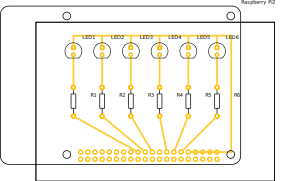
\includegraphics[height=0.4\textheight]{placafinal_pcb}
\end{figure}

\begin{figure}[H]
\centering
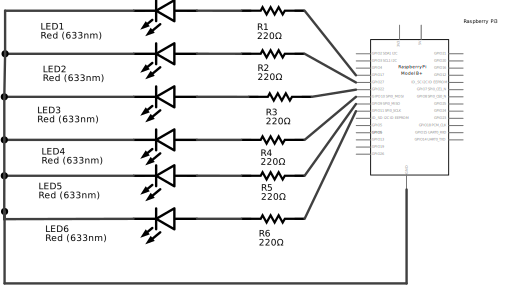
\includegraphics[height=0.4\textheight]{placafinalschematic_schem}
\end{figure}


%TODO Redmine

\end{document}
